\section{业务与数据流程}

\subsection{核心业务流程}

平台的核心业务闭环为：“打开 App 找钓点 → 判断是否可钓 → 出钓并记录 → 发布分享 → 数据反哺推荐”。

\begin{figure}[H]
  \centering
  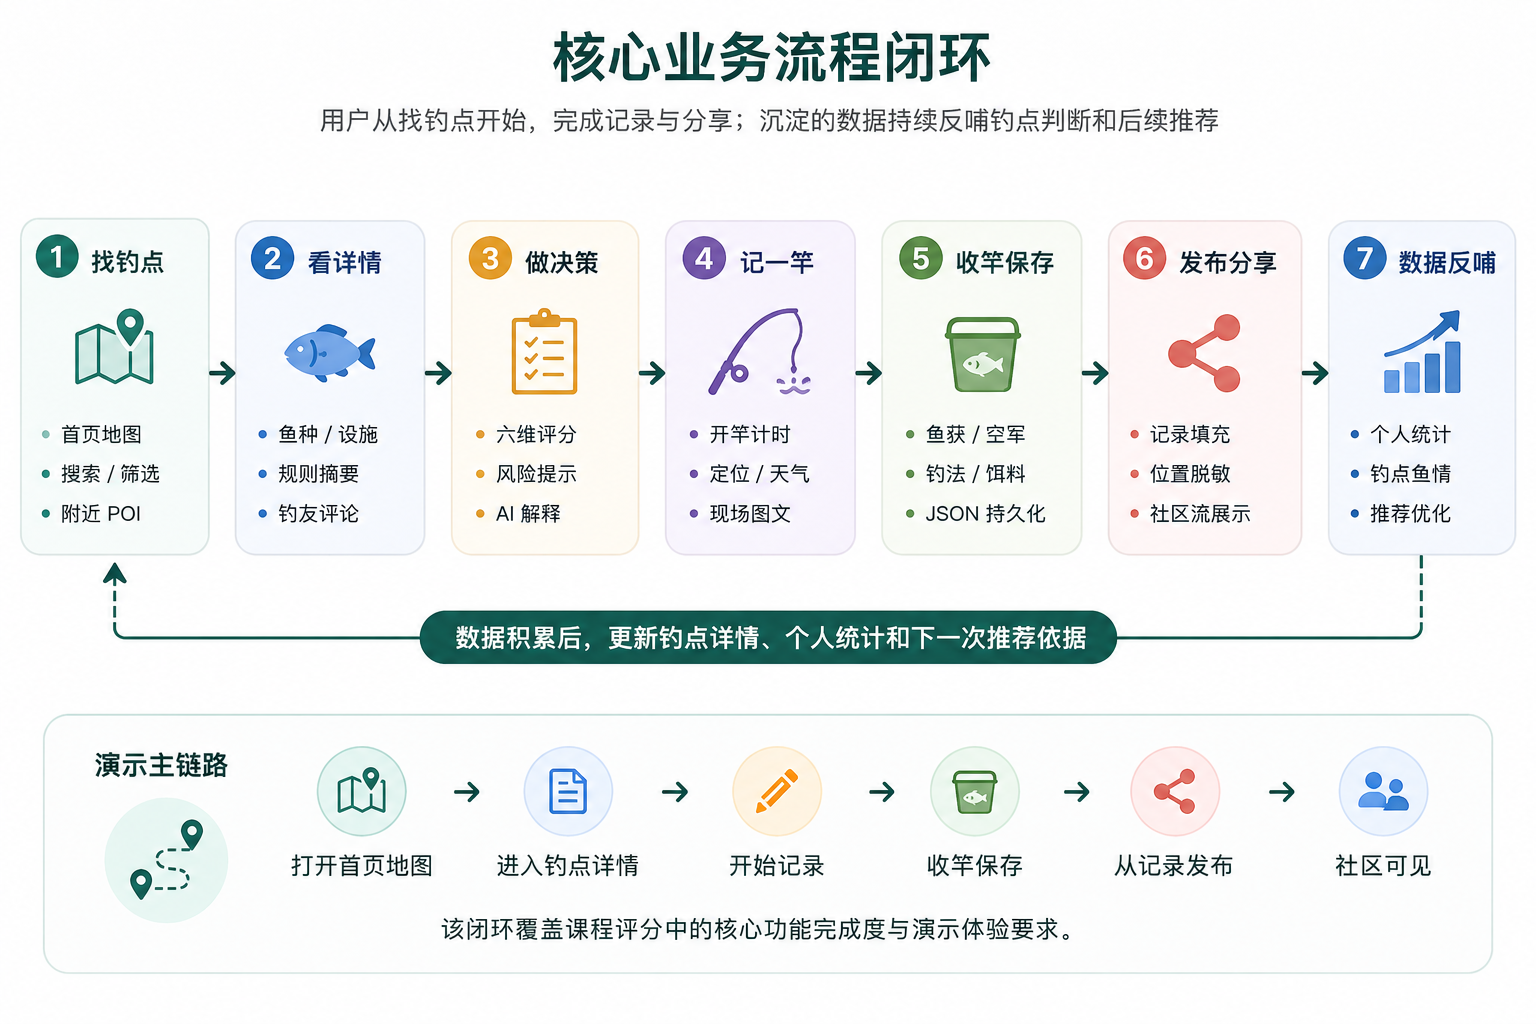
\includegraphics[width=0.85\textwidth]{figures/business_flow.png}
  \caption{核心业务流程图}
  \label{fig:biz-flow}
\end{figure}

\textbf{流程步骤说明：}

\begin{enumerate}
  \item \textbf{找钓点}：用户打开 App，地图首页根据当前位置展示附近钓点。用户可通过搜索、筛选（野钓/钓场/免费/夜钓/路亚等）缩小范围。
  \item \textbf{看详情}：点击 POI 查看钓点详情——名称、类型、距离、鱼种、收费、设施、规则摘要、近期鱼获统计和钓友评价。系统展示推荐理由、合规风险提示和天气适配情况。
  \item \textbf{做决策}：系统根据鱼情分、合规分、距离分、天气适配分、设施便利分和社交热度分计算推荐指数，对 Top 推荐结果由 DeepSeek 生成自然语言建议。禁钓/限钓/极端天气等风险优先提示。
  \item \textbf{出钓记录}：用户到达钓点后，点击“记一竿”开始计时。收竿时填写鱼获信息（鱼种、条数、重量、钓法、饵料）或标记为空军（记录原因和复盘）。天气、时间、位置由系统自动回填。
  \item \textbf{发布分享}：记录完成后可一键生成帖子发布到社区。发布时分别设置内容权限（公开/私密）和位置权限（精确/模糊/隐藏）。生成可分享的战绩卡片。
  \item \textbf{数据沉淀}：鱼获数据进入社区流和钓点详情页，成为其他用户判断该钓点的依据。用户个人主页汇总出钓统计。数据积累后提升推荐准确度。
  \item \textbf{反哺推荐}：形成“用户记录 → 数据沉淀 → 更好推荐 → 更多出钓 → 更多记录”的正向增长闭环。
\end{enumerate}

\subsection{数据流设计}

\begin{figure}[H]
  \centering
  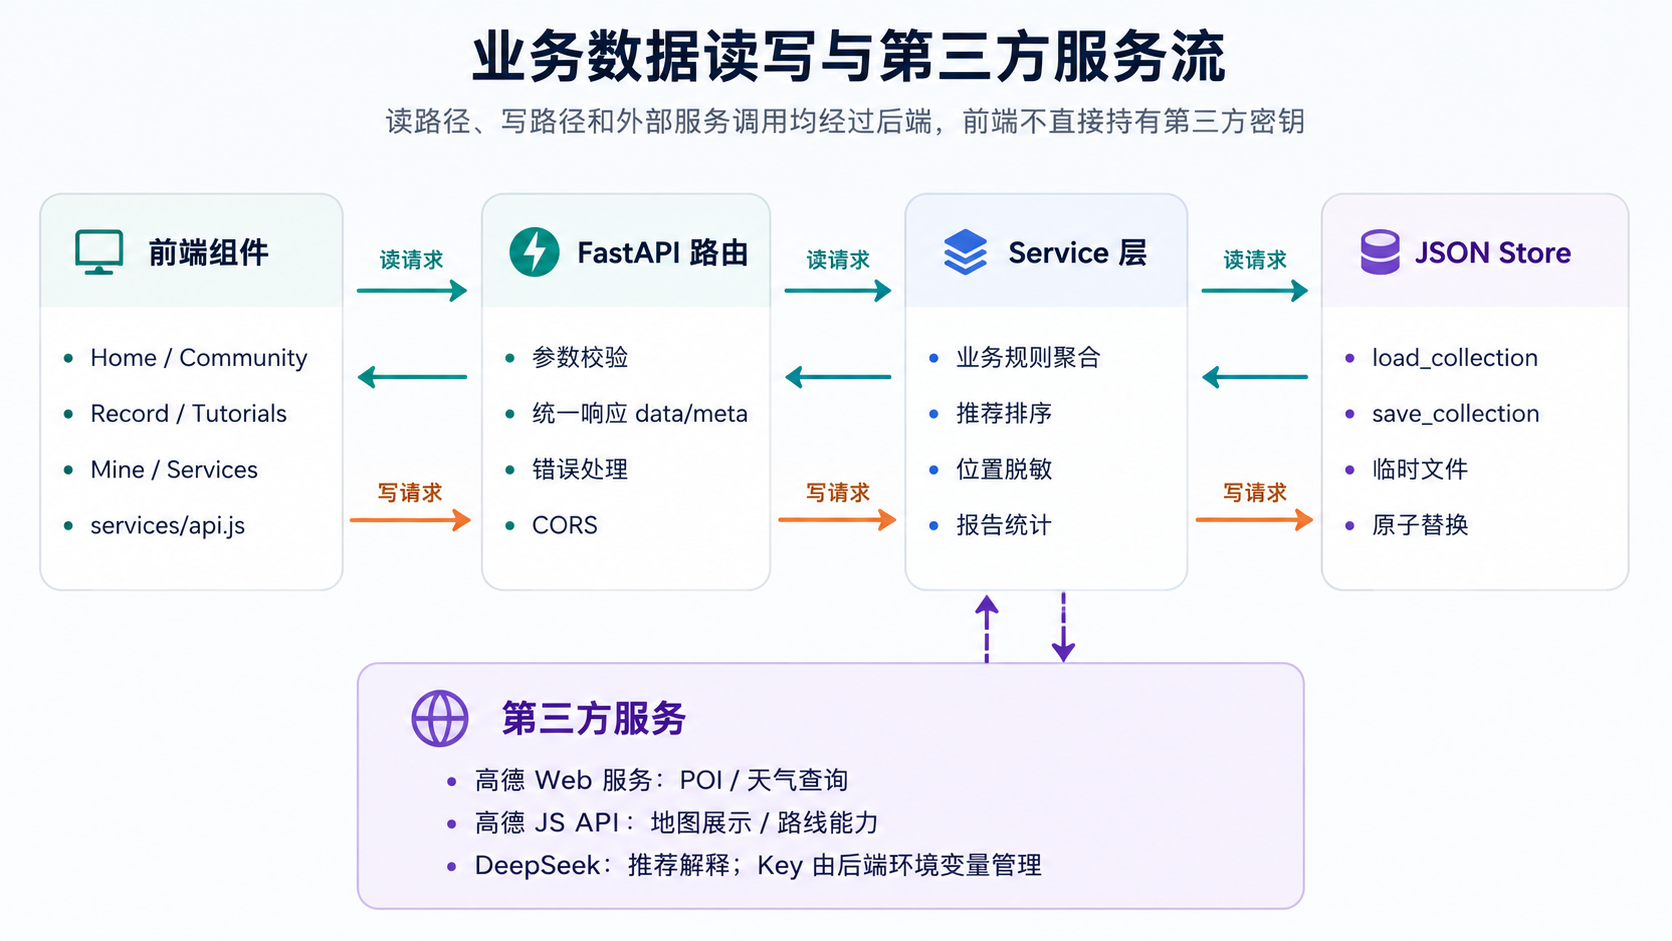
\includegraphics[width=0.85\textwidth]{figures/data_flow.png}
  \caption{数据流架构图}
  \label{fig:data-flow}
\end{figure}

\textbf{数据读写路径：}

\begin{enumerate}
  \item \textbf{读路径}：前端组件 → \texttt{api.js}（HTTP 请求）→ Vite 代理 `/api` → FastAPI 路由 → Service 层调用 \texttt{load\_collection()} → 读取 `data/*.json` → 返回结构化 JSON → 前端渲染
  \item \textbf{写路径}：前端表单提交 → \texttt{api.js} → FastAPI 路由（Pydantic 校验）→ Service 层处理业务逻辑 → \texttt{save\_collection()}（临时文件 + 原子替换）→ 返回写入结果 → 前端更新状态
  \item \textbf{第三方数据接入}：后端 Service 层封装高德 Web 服务（POI 搜索、天气查询）和 DeepSeek API 调用，前端不直接访问第三方服务。当前 MVP 阶段第三方数据以 mock 方式提供，预留真实接口结构。
\end{enumerate}

\subsection{关键数据实体关系}

\begin{table}[H]
  \centering
  \caption{核心数据实体}
  \label{tab:data-entities}
  \begin{tabularx}{\textwidth}{p{3cm}|p{4cm}|p{8cm}}
    \toprule
    \textbf{实体} & \textbf{存储位置} & \textbf{关键关联} \\
    \midrule
    FishingPOI（钓点） & \texttt{data/pois.json} & 被 CatchPost、Recommendation 引用；与高德 POI ID 关联 \\
    \hline
    CatchPost（鱼获记录） & \texttt{data/records.json} & 关联 POI（poi\_id）、用户（user\_id）、天气快照；可作为帖子来源 \\
    \hline
    Post（社区帖子） & \texttt{data/posts.json} & 可关联记录（record\_id）、POI（poi\_id）、用户（user\_id） \\
    \hline
    Recommendation（推荐） & 接口实时生成 & 引用 POI 列表、天气快照、用户偏好摘要 \\
    \hline
    WeatherSnapshot（天气） & \texttt{data/weather\_snapshots.json} & 被 Record、Recommendation 引用 \\
    \hline
    Tutorial（教程） & \texttt{data/tutorials.json} & 关联 POI（练习钓点推荐） \\
    \bottomrule
  \end{tabularx}
\end{table}

实体间核心关系：

\begin{itemize}
  \item 一条 CatchPost 隶属于一个 POI 和一个用户，携带一个天气快照
  \item 一条 Post 可选关联一条 CatchPost（从记录一键生成帖子），此时帖子可追溯到原始出钓数据
  \item 一次 Recommendation 以用户位置和偏好为输入，输出一组候选 POI 及其评分明细
  \item 当前 MVP 阶段以 JSON 文件内 \texttt{\_id} 字段实现实体引用，不引入外键约束
\end{itemize}

\subsection{当前实现状态}

当前 MVP 阶段已实现上述主流程中的关键节点：地图首页展示 POI、POI 详情查看、推荐接口返回评分与理由、记录 CRUD、帖子发布与社区流展示、个人统计汇总。数据持久化通过 JSON 原子写入实现，服务重启后数据不丢失。后续可在现有数据流基础上扩展用户系统、评论/点赞持久化和推荐算法优化。
